\documentclass[11pt,landscape]{exam}
\usepackage[margin=0.3in]{geometry}
\usepackage{multicol,tikz,graphicx}
\usetikzlibrary{shadings,decorations.pathmorphing,arrows.meta,patterns}




\begin{document}

\begin{multicols}{2}

  \begin{itemize}
    \item the color of a light wave is determined by \fillin[frequency/wavelenghth][12em] \vspace{0.5em}
    \item white: \vspace{2.5em}
    \item black: \vspace{2.5em}
    \item an object appears to be a color because it \fillin[reflects][12em] only that wavelength of light and \fillin[absorbs][12em] all the other wavelengths.
  \end{itemize}

  \vspace{7em}

  \begin{center}
    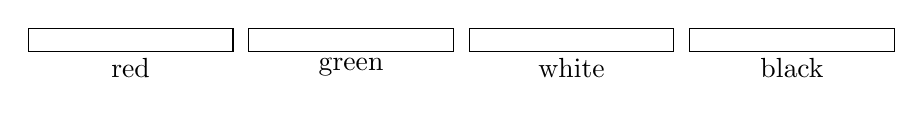
\begin{tikzpicture}
      \def\sep{2.8}
      \def\w{2.6}
      \draw[thin] (0,0) rectangle ++(\w,0.3) node[midway, below=3] {red};
      \draw[thin] (1*\sep,0) rectangle ++(\w,0.3) node[midway, below=3] {green};
      \draw[thin] (2*\sep,0) rectangle ++(\w,0.3) node[midway, below=3] {white};
      \draw[thin] (3*\sep,0) rectangle ++(\w,0.3) node[midway, below=3] {black};
    \end{tikzpicture}
  \end{center}


  \section*{Human Color Perception}

  \hfill 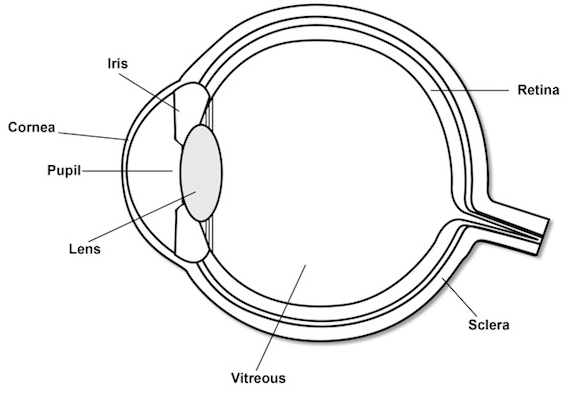
\includegraphics[width=4.5cm]{eye} \hfill{}

  \begin{itemize}
    \item the back of your eye is called the \fillin[retina][8em]. \vspace{0.5em}
    \item rods: \vspace{2em}
    \item cones: \vspace{2em}
    \item the three types of cones in your eye percieve the colors \\\fillin[red][7em], \fillin[green][7em], and \fillin[blue][7em].
  \end{itemize}


  \columnbreak

  \subsection*{Additive Color Mixing}

  \begin{itemize}
    \item Different colored lights are \fillin[added][8em] to each other.  \vspace{0.5em}
    \item the three three additive primary colors are \\\fillin[red][7em], \fillin[green][7em], and \fillin[blue][7em].
    
    \begin{center}
        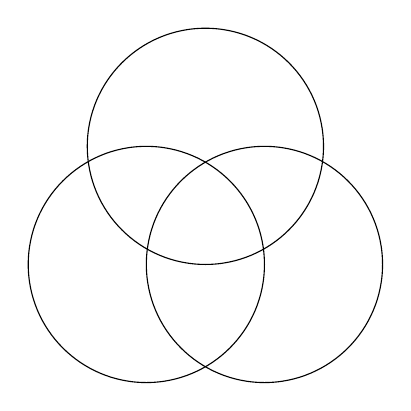
\begin{tikzpicture}
          \def\sep{.75}
          \draw (0,0) circle (1.5);
          \draw (-\sep,-2*\sep) circle (1.5);
          \draw ( \sep,-2*\sep) circle (1.5);
      \end{tikzpicture}
    \end{center}

    \item Mixing all the colors additively gives \fillin[white][8em].
  \end{itemize}


  \vspace{2em}

  \subsection*{Subtractive Color Mixing}

  \begin{itemize}
    \item Different colored filters or pigments \fillin[absorb][6em] or \fillin[subtract][6em] some colors of light. \vspace{0.5em}
    \item the three three subtractive primary colors are \\\fillin[cyan][7em], \fillin[magenta][7em], and \fillin[yellow][7em]. \vspace{0.5em}
    \item Mixing all the colors subtractively gives \fillin[black][7em].
  \end{itemize}


\end{multicols}

\end{document}